% Chapter 8 Roadmap Diagram
\begin{figure}[ht]
\centering
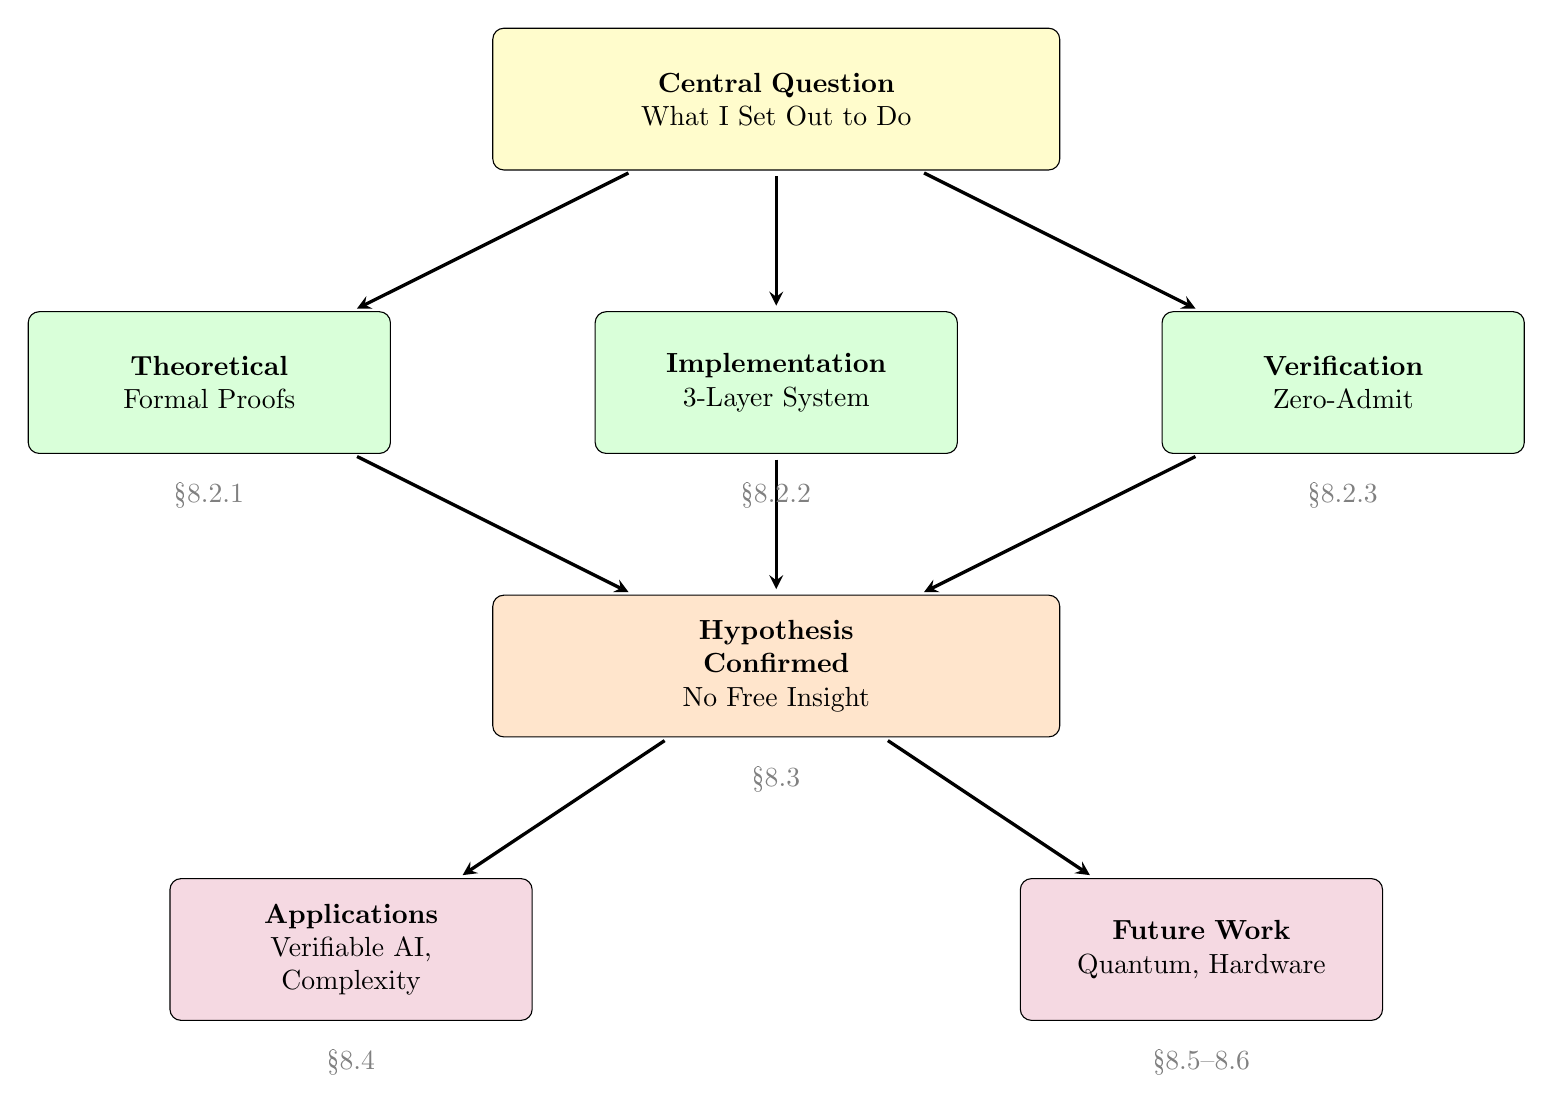
\begin{tikzpicture}[scale=1.8, 
    node distance=3cm,
    box/.style={draw, rounded corners, minimum width=4.6cm, minimum height=1.8cm, align=center, fill=blue!10},
    arrow/.style={->, very thick, >=stealth}
]
    % Central question
    \node[box, fill=yellow!20, minimum width=7.2cm, align=center, text width=3.5cm, font=\normalsize] (q) at (0,0) {\textbf{Central Question}\\What I Set Out to Do};
    
    % Three goals
    \node[box, fill=green!15, align=center, text width=3.5cm, font=\normalsize] (t) at (-4,-2) {\textbf{Theoretical}\\Formal Proofs};
    \node[box, fill=green!15, align=center, text width=3.5cm, font=\normalsize] (i) at (0,-2) {\textbf{Implementation}\\3-Layer System};
    \node[box, fill=green!15, align=center, text width=3.5cm, font=\normalsize] (v) at (4,-2) {\textbf{Verification}\\Zero-Admit};
    
    % Hypothesis confirmation
    \node[box, fill=orange!20, minimum width=7.2cm, align=center, text width=3.5cm, font=\normalsize] (h) at (0,-4) {\textbf{Hypothesis Confirmed}\\No Free Insight};
    
    % Applications and Future
    \node[box, fill=purple!15, align=center, text width=3.5cm, font=\normalsize] (a) at (-3,-6) {\textbf{Applications}\\Verifiable AI, Complexity};
    \node[box, fill=purple!15, align=center, text width=3.5cm, font=\normalsize] (f) at (3,-6) {\textbf{Future Work}\\Quantum, Hardware};
    
    % Arrows
    \draw[arrow, shorten >=2pt, shorten <=2pt] (q) -- (t);
    \draw[arrow, shorten >=2pt, shorten <=2pt] (q) -- (i);
    \draw[arrow, shorten >=2pt, shorten <=2pt] (q) -- (v);
    \draw[arrow, shorten >=2pt, shorten <=2pt] (t) -- (h);
    \draw[arrow, shorten >=2pt, shorten <=2pt] (i) -- (h);
    \draw[arrow, shorten >=2pt, shorten <=2pt] (v) -- (h);
    \draw[arrow, shorten >=2pt, shorten <=2pt] (h) -- (a);
    \draw[arrow, shorten >=2pt, shorten <=2pt] (h) -- (f);
    
    % Section annotations
    \node[font=\normalsize, gray] at (-4,-2.8) {§8.2.1};
    \node[font=\normalsize, gray] at (0,-2.8) {§8.2.2};
    \node[font=\normalsize, gray] at (4,-2.8) {§8.2.3};
    \node[font=\normalsize, gray] at (0,-4.8) {§8.3};
    \node[font=\normalsize, gray] at (-3,-6.8) {§8.4};
    \node[font=\normalsize, gray] at (3,-6.8) {§8.5--8.6};
\end{tikzpicture}
\caption{Chapter 8 roadmap: From central question through contributions to confirmed hypothesis and future directions.}
\label{fig:ch8_roadmap}

\paragraph{Understanding Figure~\ref{fig:ch8_roadmap}:}

This \textbf{roadmap diagram} visualizes Chapter 8's structure: starting with the central research question, flowing through three categories of contributions (theoretical, implementation, verification), converging on hypothesis confirmation, and branching to applications and future work.

\textbf{Visual elements:}
\begin{itemize}
    \item \textbf{Top yellow box:} ``Central Question: What I Set Out to Do''---the thesis's motivating question (\textit{What if structural insight were treated as a conserved resource?}).
    \item \textbf{Three green boxes (middle):} The three categories of contributions:
    \begin{itemize}
        \item \textbf{Theoretical (left):} Formal proofs (5-tuple formalization, $\mu$-bit currency, No Free Insight theorem, no-signaling theorem).
        \item \textbf{Implementation (center):} 3-layer system (Coq kernel, Python VM, Verilog RTL with isomorphism invariant).
        \item \textbf{Verification (right):} Zero-admit standard (206 proofs, 0 admits, 0 global axioms, Bell inequality foundation proven, Inquisitor enforcement).
    \end{itemize}
    \item \textbf{Orange box (center-bottom):} ``Hypothesis Confirmed: No Free Insight''---the thesis's central claim, validated by all three contribution categories.
    \item \textbf{Two purple boxes (bottom):} Future directions:
    \begin{itemize}
        \item \textbf{Applications (left):} Verifiable AI, complexity theory, physics bridges.
        \item \textbf{Future Work (right):} Quantum extension, hardware realization, distributed execution.
    \end{itemize}
    \item \textbf{Arrows:} Flow from central question $\to$ three contributions $\to$ hypothesis confirmation $\to$ applications/future work.
    \item \textbf{Section annotations (gray text):} Each box has a reference to the corresponding section (e.g., §8.2.1, §8.3, §8.4).
\end{itemize}

\textbf{Key insight visualized:} The roadmap shows that the thesis is \textit{structured around validation}: starting with a question, executing a systematic plan (theory, implementation, verification), confirming the hypothesis, and identifying next steps. The three contribution categories are \textit{independent lines of evidence} that converge on the same conclusion.

\textbf{How to read this diagram:}
\begin{enumerate}
    \item Start at the top: The central question (``What if structure were a conserved resource?'').
    \item Middle layer: Three distinct approaches to answering the question: mathematical proof (Coq theorems), executable implementation (3 layers), rigorous verification (zero admits).
    \item Center-bottom: All three contributions converge on ``Hypothesis Confirmed''.
    \item Bottom: The confirmed hypothesis enables applications (AI, complexity) and future extensions (quantum, hardware).
\end{enumerate}

\textbf{Role in thesis:} This roadmap orients the reader at the start of the conclusion, summarizing the thesis's logical flow. It emphasizes \textit{convergence}---the hypothesis is not just proven (Coq), but also implemented (3 layers) and verified (zero admits). This three-pronged confirmation is the thesis's core strength.

\end{figure}

\section{What I Set Out to Do}

\subsection{The Central Claim}

At the beginning of this thesis, I posed a question:
\begin{quote}
    \textit{What if structural insight---the knowledge that makes hard problems easy---were treated as a real, conserved, costly resource?}
\end{quote}

I claimed that this perspective would yield a coherent computational model with:
\begin{itemize}
    \item Formally provable properties (no hand-waving)
    \item Executable implementations (not just paper proofs)
    \item Connections to fundamental physics (not just analogies)
\end{itemize}

This conclusion evaluates whether I achieved these goals and clarifies which claims are proved, which are implemented, and which remain empirical hypotheses. The guiding standard is rebuildability: a reader should be able to reconstruct the model and its evidence from the thesis text alone.

\subsection{How to Read This Chapter}

Section 8.2 summarizes my theoretical, implementation, and verification contributions. Section 8.3 assesses whether the central hypothesis is confirmed. Sections 8.4--8.6 discuss applications, open problems, and future directions.

\textbf{For readers short on time}: Section 8.3 ("The Thiele Machine Hypothesis: Confirmed") provides the essential verdict.

\section{Summary of Contributions}

This thesis has presented the Thiele Machine, a computational model that treats structural information as a conserved, costly resource. My contributions are:

\subsection{Theoretical Contributions}

\begin{enumerate}
    \item \textbf{The 5-Tuple Formalization}: I defined the Thiele Machine as $T = (S, \Pi, A, R, L)$ with explicit state space, partition graph, axiom sets, transition rules, and logic engine. This formalization enables precise mathematical reasoning about structural computation.
    
    \item \textbf{The $\mu$-bit Currency}: I introduced the $\mu$-bit as the atomic unit of structural information cost. The ledger is proven monotone, and its growth lower-bounds irreversible bit events; this ties structural accounting to an operational notion of irreversibility.
    
    \item \textbf{The No Free Insight Theorem}: I proved that strengthening certification predicates requires explicit, charged revelation events. This establishes that "free" structural information is impossible within the model’s rules.
    
    \item \textbf{Observational No-Signaling}: I proved that operations on one module cannot affect the observables of unrelated modules—a computational analog of Bell locality.
\end{enumerate}
These theoretical components map to concrete Coq artifacts: \path{VMState.v} and \path{VMStep.v} define the formal machine, \path{MuLedgerConservation.v} proves monotonicity and irreversibility bounds, and \path{NoFreeInsight.v} formalizes the impossibility claim. The contribution is therefore not just conceptual; it is encoded in machine-checked definitions.

% Theoretical Contributions Diagram
\begin{figure}[ht]
\centering
\begin{tikzpicture}[scale=1.8, 
    node distance=2.5cm,
    box/.style={draw, rounded corners, minimum width=5.4cm, minimum height=1.6cm, align=center, fill=blue!10},
    arrow/.style={->, very thick, >=stealth}
]
    % Four main contributions
    \node[box, fill=yellow!20, align=center, text width=3.5cm, font=\normalsize] (tuple) at (0,0) {\textbf{5-Tuple Formalization}\\$T = (S, \Pi, A, R, L)$};
    \node[box, fill=green!15, align=center, text width=3.5cm, font=\normalsize] (mu) at (5,0) {\textbf{$\mu$-bit Currency}\\Monotone Ledger};
    \node[box, fill=orange!15, align=center, text width=3.5cm, font=\normalsize] (nfi) at (0,-2.5) {\textbf{No Free Insight}\\Impossibility Theorem};
    \node[box, fill=purple!15, align=center, text width=3.5cm, font=\normalsize] (nosig) at (5,-2.5) {\textbf{No-Signaling}\\Bell Locality};
    
    % Central node
    \node[draw, circle, fill=red!20, minimum size=1.5cm, align=center, text width=3.5cm] (center) at (2.5,-1.25) {\textbf{Coq}\\Verified};
    
    % Arrows to center
    \draw[arrow, shorten >=2pt, shorten <=2pt] (tuple) -- (center);
    \draw[arrow, shorten >=2pt, shorten <=2pt] (mu) -- (center);
    \draw[arrow, shorten >=2pt, shorten <=2pt] (nfi) -- (center);
    \draw[arrow, shorten >=2pt, shorten <=2pt] (nosig) -- (center);
    
    % File annotations
    \node[font=\normalsize, gray, below=0.3cm of tuple, sloped, pos=0.5, font=\small, yshift=-6pt] {VMState.v, VMStep.v};
    \node[font=\normalsize, gray, below=0.3cm of mu, sloped, pos=0.5, font=\small, yshift=-6pt] {MuLedgerConservation.v};
    \node[font=\normalsize, gray, below=0.3cm of nfi, above, pos=0.5, font=\small, yshift=6pt] {NoFreeInsight.v};
    \node[font=\normalsize, gray, below=0.3cm of nosig, above, pos=0.5, font=\small, yshift=6pt] {KernelPhysics.v};
\end{tikzpicture}
\caption{Theoretical contributions: Four core results, all machine-verified in Coq.}
\label{fig:theoretical_contributions}

\paragraph{Understanding Figure~\ref{fig:theoretical_contributions}:}

This \textbf{theoretical contributions diagram} visualizes the four foundational results of the thesis, all formally proven in Coq and converging on machine verification.

\textbf{Visual elements:}
\begin{itemize}
    \item \textbf{Four boxes (corners):} The four core theoretical contributions:
    \begin{itemize}
        \item \textbf{5-Tuple Formalization (yellow, top-left):} The Thiele Machine definition $T = (S, \Pi, A, R, L)$ (State space, Partition graph, Axiom sets, Transition rules, Logic engine). File: \texttt{VMState.v}, \texttt{VMStep.v}.
        \item \textbf{$\mu$-bit Currency (green, top-right):} The $\mu$-ledger as a conserved resource, proven monotone (never decreases) and lower-bounding irreversible operations. File: \texttt{MuLedgerConservation.v}.
        \item \textbf{No Free Insight (orange, bottom-left):} Impossibility theorem stating that strengthening certification predicates requires explicit revelation events. File: \texttt{NoFreeInsight.v}.
        \item \textbf{No-Signaling (purple, bottom-right):} Computational Bell locality---operations on module A cannot affect observables of module B. File: \texttt{KernelPhysics.v}.
    \end{itemize}
    \item \textbf{Central red circle:} Labeled ``Coq Verified''---all four contributions are machine-checked theorems (not hand-proofs).
    \item \textbf{Arrows:} From each of the four boxes to the central circle, showing convergence on formal verification.
    \item \textbf{File annotations (gray text below boxes):} Each contribution lists the Coq file containing the formal proof (e.g., \texttt{VMState.v}, \texttt{MuLedgerConservation.v}).
\end{itemize}

\textbf{Key insight visualized:} The diagram emphasizes that these contributions are not \textit{conceptual claims}---they are \textbf{machine-checked theorems}. The central red circle (``Coq Verified'') is the thesis's seal of rigor: every arrow represents a formal proof that Coq's type-checker has validated. The file annotations make the claims \textit{auditable}---readers can inspect the exact Coq code.

\textbf{How to read this diagram:}
\begin{enumerate}
    \item \textbf{Four corners:} Each box represents a major theoretical result. These are \textit{independent} contributions (you could prove one without the others).
    \item \textbf{Central circle:} All four contributions are \textit{verified} in Coq. This means:
    \begin{itemize}
        \item No informal gaps in the proofs.
        \item No hidden assumptions (zero global axioms; documented assumptions use Section/Context pattern).
        \item No unfinished proof obligations (zero admits).
    \end{itemize}
    \item \textbf{File annotations:} These provide \textit{traceability}. Readers can navigate to \path{coq/kernel/VMState.v} and see the exact definition of $T = (S, \Pi, A, R, L)$.
\end{enumerate}

\textbf{Role in thesis:} This diagram summarizes the theoretical contributions in Section 8.2.1. It distinguishes the Thiele Machine from \textit{informal computational models} (e.g., those described only in prose or pseudocode). Every claim is \textit{proven}, not \textit{asserted}. The diagram provides a high-level map of the formal artifacts, with file references anchoring each claim to concrete Coq code.

\end{figure}

\subsection{Implementation Contributions}

\begin{enumerate}
    \item \textbf{3-Layer Isomorphism}: I implemented the model across three layers:
    \begin{itemize}
        \item Coq formal kernel (zero admits, zero axioms)
        \item Python reference VM with receipts and trace replay
        \item Verilog RTL suitable for synthesis
    \end{itemize}
    All three layers produce identical state projections for any instruction trace, with the projection chosen to match the gate being exercised. For compute traces the gate compares registers and memory; for partition traces it compares canonicalized module regions. The extracted runner provides a superset snapshot (pc, $\mu$, err, regs, mem, CSRs, graph) that can be used when a gate needs a broader view.
    
    \item \textbf{18-Instruction ISA}: I defined a minimal instruction set sufficient for partition-native computation. The ISA is intentionally small so that each opcode has a clear semantic role: structure creation, structure modification, certification, computation, and control.
    \begin{itemize}
        \item Structural: PNEW, PSPLIT, PMERGE, PDISCOVER
        \item Logical: LASSERT, LJOIN
        \item Certification: REVEAL, EMIT
        \item Compute: XFER, XOR\_LOAD, XOR\_ADD, XOR\_SWAP, XOR\_RANK
        \item Control: PYEXEC, ORACLE\_HALTS, HALT, CHSH\_TRIAL, MDLACC
    \end{itemize}
    
    \item \textbf{The Inquisitor}: I built automated verification tooling that enforces zero-admit discipline and runs the isomorphism gates.
\end{enumerate}
The implementations are organized so they can be audited against the formal kernel: the Coq layer is under \path{coq/kernel/}, the Python VM under \path{thielecpu/}, and the RTL under \path{thielecpu/hardware/}. The isomorphism tests consume traces that exercise all three and compare their observable projections.

% 3-Layer Implementation Diagram
\begin{figure}[ht]
\centering
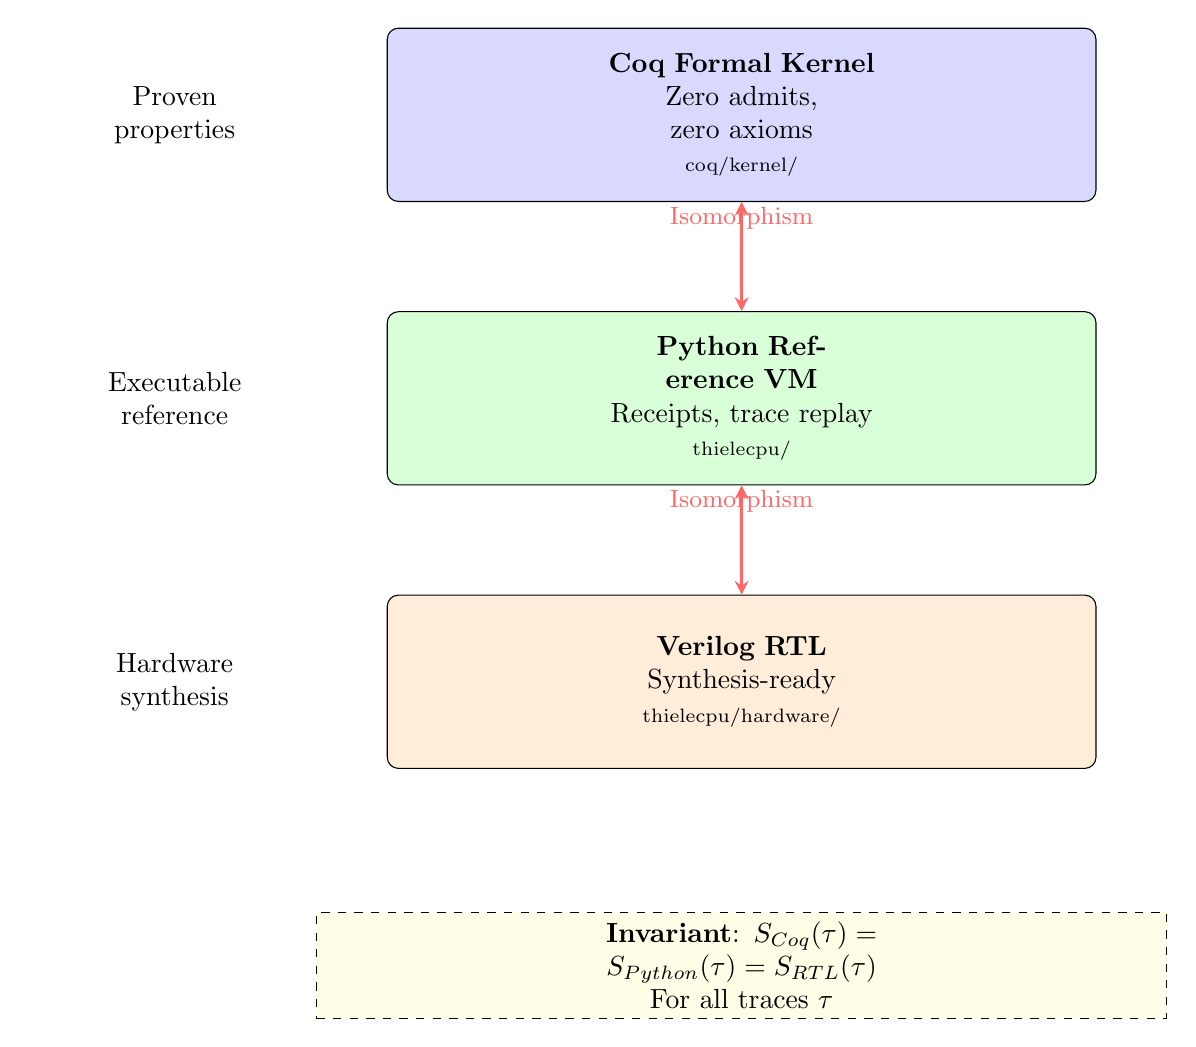
\begin{tikzpicture}[scale=1.8, 
    node distance=2.5cm,
    layer/.style={draw, rounded corners, minimum width=9.0cm, minimum height=2.2cm, align=center},
    arrow/.style={<->, very thick, >=stealth}
]
    % Three layers
    \node[layer, fill=blue!15, align=center, text width=3.5cm] (coq) at (0,2) {\textbf{Coq Formal Kernel}\\Zero admits, zero axioms\\{\scriptsize coq/kernel/}};
    \node[layer, fill=green!15, align=center, text width=3.5cm] (py) at (0,0) {\textbf{Python Reference VM}\\Receipts, trace replay\\{\scriptsize thielecpu/}};
    \node[layer, fill=orange!15, align=center, text width=3.5cm] (rtl) at (0,-2) {\textbf{Verilog RTL}\\Synthesis-ready\\{\scriptsize thielecpu/hardware/}};
    
    % Isomorphism arrows
    \draw[arrow, red!60] (coq) -- node[right, font=\normalsize, above, yshift=6pt, pos=0.5, font=\small] {Isomorphism} (py);
    \draw[arrow, red!60] (py) -- node[right, font=\normalsize, above, yshift=6pt, pos=0.5, font=\small] {Isomorphism} (rtl);
    
    % Invariant box
    \node[draw, dashed, fill=yellow!10, minimum width=10.8cm, align=center, text width=3.5cm] at (0,-4) {
        \textbf{Invariant}: $S_{\text{Coq}}(\tau) = S_{\text{Python}}(\tau) = S_{\text{RTL}}(\tau)$\\
        For all traces $\tau$
    };
    
    % Left annotations
    \node[font=\normalsize, align=right, align=center, text width=3.5cm] at (-4,2) {Proven\\properties};
    \node[font=\normalsize, align=right, align=center, text width=3.5cm] at (-4,0) {Executable\\reference};
    \node[font=\normalsize, align=right, align=center, text width=3.5cm] at (-4,-2) {Hardware\\synthesis};
\end{tikzpicture}
\caption{3-layer implementation architecture with isomorphism invariant preserved across all levels.}
\label{fig:three_layer_impl}

\paragraph{Understanding Figure~\ref{fig:three_layer_impl}:}

This \textbf{3-layer implementation diagram} visualizes the architectural structure of the Thiele Machine: three independent implementations (Coq, Python, Verilog) bound by a single isomorphism invariant.

\textbf{Visual elements:}
\begin{itemize}
    \item \textbf{Three horizontal boxes (layers):}
    \begin{itemize}
        \item \textbf{Top (blue):} Coq Formal Kernel---zero admits, zero axioms. Directory: \texttt{coq/kernel/}. This is the \textit{ground truth} (proven correct by Coq's type-checker).
        \item \textbf{Middle (green):} Python Reference VM---receipts, trace replay. Directory: \texttt{thielecpu/}. This is the \textit{executable reference} (fast prototyping, debugging, empirical validation).
        \item \textbf{Bottom (orange):} Verilog RTL---synthesis-ready. Directory: \texttt{thielecpu/hardware/}. This is the \textit{hardware implementation} (FPGA deployment, silicon target).
    \end{itemize}
    \item \textbf{Red bidirectional arrows:} Labeled ``Isomorphism'' connecting adjacent layers. These represent the claim: $S_{\text{Coq}}(\tau) = S_{\text{Python}}(\tau) = S_{\text{RTL}}(\tau)$ for all traces $\tau$.
    \item \textbf{Left annotations (gray text):} Describe the role of each layer:
    \begin{itemize}
        \item Coq: ``Proven properties'' (formal guarantees).
        \item Python: ``Executable reference'' (operational semantics).
        \item RTL: ``Hardware synthesis'' (physical realization).
    \end{itemize}
    \item \textbf{Bottom dashed yellow box:} ``Invariant: $S_{\text{Coq}}(\tau) = S_{\text{Python}}(\tau) = S_{\text{RTL}}(\tau)$ for all traces $\tau$''---the \textbf{isomorphism claim}.
\end{itemize}

\textbf{Key insight visualized:} The three layers are not merely ``compatible''---they are \textit{isomorphic}. For any instruction trace $\tau$, executing on all three layers produces \textit{identical} final states (modulo observable projections). This means:
\begin{itemize}
    \item \textbf{Coq guarantees formal correctness:} Theorems proven in Coq \textit{hold} in the Python VM and RTL.
    \item \textbf{Python enables empirical testing:} Experiments in Python \textit{validate} the formal model.
    \item \textbf{RTL allows hardware deployment:} Synthesizing to FPGA/ASIC \textit{preserves} the formal semantics.
\end{itemize}

\textbf{How to read this diagram:}
\begin{enumerate}
    \item \textbf{Top layer (Coq):} This is the \textit{source of truth}. Every theorem proven here is \textit{certain} (machine-checked, zero admits).
    \item \textbf{Arrows (isomorphism):} The red arrows claim that Python and RTL \textit{exactly match} the Coq semantics. This is not an assumption---it's a \textit{tested claim} (see Chapter 6 isomorphism gates).
    \item \textbf{Bottom layer (RTL):} Hardware synthesis preserves the formal properties proven in Coq. If a theorem holds in Coq, it holds in the synthesized FPGA bitstream.
    \item \textbf{Yellow box (invariant):} The mathematical statement of the isomorphism. $S_{\text{Coq}}(\tau)$ is the state produced by the Coq extracted runner, $S_{\text{Python}}(\tau)$ is the Python VM's state, $S_{\text{RTL}}(\tau)$ is the RTL simulation's state. For \textit{all} traces $\tau$, these three states are equal (under the appropriate projection).
\end{enumerate}

\textbf{Role in thesis:} This diagram illustrates the implementation contributions (Section 8.2.2). The 3-layer architecture ensures that formal proofs are not \textit{detached from reality}---they govern the behavior of executable code and synthesizable hardware. The isomorphism invariant is the \textbf{bridge} between theory (Coq) and practice (Python/RTL).

\end{figure}

\subsection{Verification Contributions}

\begin{enumerate}
    \item \textbf{Zero-Admit Campaign}: The Coq formalization contains a complete proof tree with no admits and no axioms beyond foundational logic. This is enforced by the verification tooling and guarantees that every theorem is fully discharged within the formal system.
    
    \item \textbf{Key Proven Theorems}:
    \begin{center}
    \resizebox{0.9\textwidth}{!}{
    \begin{tabular}{|l|l|}
    \hline
    \textbf{Theorem} & \textbf{Property} \\
    \hline
    \texttt{observational\_no\_signaling} & Locality \\
    \texttt{mu\_conservation\_kernel} & Single-step monotonicity \\
    \texttt{run\_vm\_mu\_conservation} & Multi-step conservation \\
    \texttt{no\_free\_insight\_general} & Impossibility \\
    \path{nonlocal_correlation_requires_revelation} & Supra-quantum certification \\
    \texttt{kernel\_conservation\_mu\_gauge} & Gauge invariance \\
    \hline
    \end{tabular}
    }
    \end{center}
    
    \item \textbf{Falsifiability}: Every theorem includes an explicit falsifier specification. If a counterexample exists, it would refute the theorem and identify the precise assumption that failed.
\end{enumerate}
The theorem names in the table correspond to statements in the Coq kernel (for example, \texttt{observational\_no\_signaling} in \path{KernelPhysics.v} and \path{nonlocal_correlation_requires_revelation} in \path{RevelationRequirement.v}). This explicit mapping is what makes the verification story reproducible.

% Verification Architecture Diagram
\begin{figure}[ht]
\centering
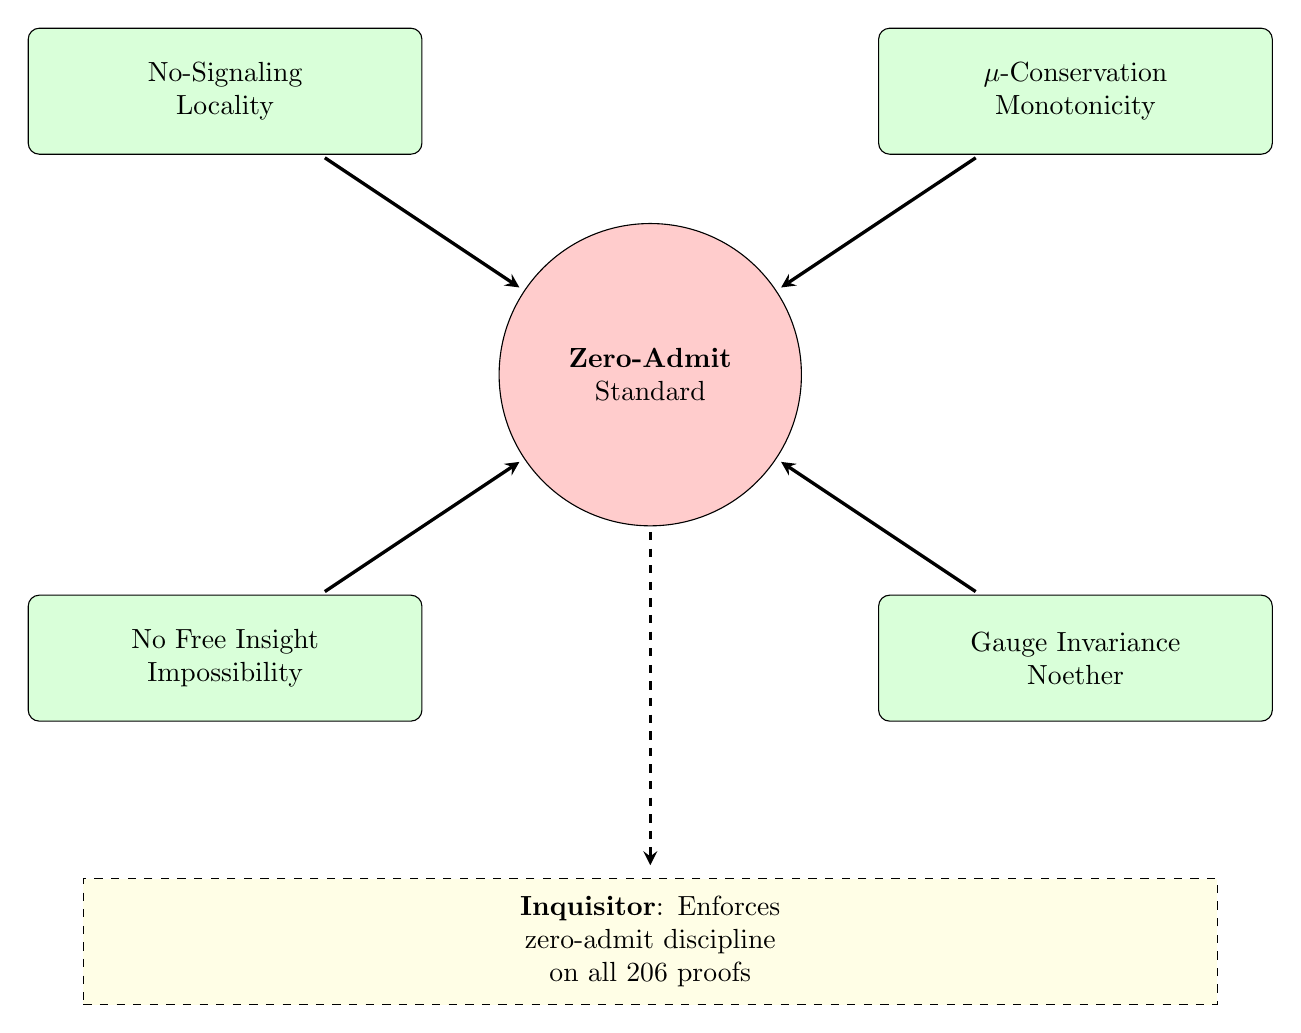
\begin{tikzpicture}[scale=1.8, 
    node distance=2.5cm,
    box/.style={draw, rounded corners, minimum width=5.0cm, minimum height=1.6cm, align=center, fill=blue!10},
    arrow/.style={->, very thick, >=stealth}
]
    % Zero-admit standard at center
    \node[draw, circle, fill=red!20, minimum size=2cm, align=center, text width=3.5cm] (zero) at (0,0) {\textbf{Zero-Admit}\\Standard};
    
    % Theorems around
    \node[box, fill=green!15, align=center, text width=3.5cm, font=\normalsize] (nosig) at (-3,2) {No-Signaling\\Locality};
    \node[box, fill=green!15, align=center, text width=3.5cm, font=\normalsize] (mucons) at (3,2) {$\mu$-Conservation\\Monotonicity};
    \node[box, fill=green!15, align=center, text width=3.5cm, font=\normalsize] (nfi) at (-3,-2) {No Free Insight\\Impossibility};
    \node[box, fill=green!15, align=center, text width=3.5cm, font=\normalsize] (gauge) at (3,-2) {Gauge Invariance\\Noether};
    
    % Arrows
    \draw[arrow, shorten >=2pt, shorten <=2pt] (nosig) -- (zero);
    \draw[arrow, shorten >=2pt, shorten <=2pt] (mucons) -- (zero);
    \draw[arrow, shorten >=2pt, shorten <=2pt] (nfi) -- (zero);
    \draw[arrow, shorten >=2pt, shorten <=2pt] (gauge) -- (zero);
    
    % Inquisitor
    \node[draw, dashed, fill=yellow!10, minimum width=14.4cm, minimum height=1.6cm, align=center, text width=3.5cm] at (0,-4) {\textbf{Inquisitor}: Enforces zero-admit discipline on all 206 proofs};
    
    % Arrow from zero to inquisitor
    \draw[arrow, dashed, shorten >=2pt, shorten <=2pt] (zero) -- (0,-3.5);
\end{tikzpicture}
\caption{Verification architecture: All theorems held to zero-admit standard, enforced by Inquisitor.}
\label{fig:verification_arch}

\paragraph{Understanding Figure~\ref{fig:verification_arch}:}

This \textbf{verification architecture diagram} visualizes the zero-admit discipline: all theorems converge on a central standard (zero admits, zero axioms), with enforcement by the Inquisitor tool.

\textbf{Visual elements:}
\begin{itemize}
    \item \textbf{Central red circle:} Labeled ``Zero-Admit Standard''---the thesis's verification policy (no \texttt{admit}, no axioms beyond foundational logic).
    \item \textbf{Four green boxes (surrounding):} Four representative theorems:
    \begin{itemize}
        \item \textbf{No-Signaling (top-left):} \texttt{observational\_no\_signaling} theorem proving computational Bell locality.
        \item \textbf{$\mu$-Conservation (top-right):} \texttt{mu\_conservation\_kernel} (single-step) and \texttt{run\_vm\_mu\_conservation} (multi-step) theorems proving ledger monotonicity.
        \item \textbf{No Free Insight (bottom-left):} \texttt{no\_free\_insight\_general} theorem proving impossibility of free structural revelation.
        \item \textbf{Gauge Invariance (bottom-right):} \texttt{kernel\_conservation\_mu\_gauge} theorem proving Noether-like symmetry.
    \end{itemize}
    \item \textbf{Arrows:} From each theorem box to the central circle, showing that all theorems \textit{satisfy} the zero-admit standard.
    \item \textbf{Bottom yellow dashed box:} ``Inquisitor: Enforces zero-admit discipline on all 206 proofs''---the automated tool that scans the Coq codebase and rejects any file containing \texttt{admit} or unapproved axioms.
    \item \textbf{Dashed arrow:} From the central circle to the Inquisitor box, showing that the standard is \textit{enforced} automatically.
\end{itemize}

\textbf{Key insight visualized:} The zero-admit standard is not a \textit{guideline}---it's a \textbf{CI-enforced invariant}. Every proof in the Coq kernel (206 total) must be \textit{complete} (no \texttt{admit}), \textit{foundational} (no axioms beyond Coq's base logic), and \textit{auditable} (verified by the Inquisitor tool). This ensures that theorems are not ``90\% proven''---they are \textit{fully discharged}.

\textbf{How to read this diagram:}
\begin{enumerate}
    \item \textbf{Central circle:} The zero-admit standard is the thesis's \textit{verification policy}. It applies to \textit{all} theorems, not just a select few.
    \item \textbf{Four boxes:} Representative examples of major theorems. Each has been proven to the zero-admit standard (no \texttt{admit}, no axioms).
    \item \textbf{Arrows:} Show that the theorems \textit{satisfy} the standard. This is not assumed---it's \textit{checked} by Coq's type-checker.
    \item \textbf{Inquisitor (bottom):} The enforcement mechanism. Before every commit, the Inquisitor scans all Coq files and rejects any containing \texttt{admit} or unapproved axioms. This is a \textit{CI gate}---the codebase cannot be merged if the standard is violated.
\end{enumerate}

\textbf{Role in thesis:} This diagram illustrates the verification contributions (Section 8.2.3). The zero-admit campaign ensures that the thesis's formal claims are \textit{trustworthy}. Unlike informal proofs (which may contain gaps), the Coq proofs are \textit{machine-checked and complete}. The Inquisitor provides continuous enforcement, preventing regression (e.g., a developer adding \texttt{admit} to bypass a difficult subgoal). The diagram emphasizes \textit{rigor} as a continuous process, not a one-time audit.

\end{figure}

\section{The Thiele Machine Hypothesis: Confirmed}

I set out to test the hypothesis:
\begin{quote}
\textit{There is no free insight. Structure must be paid for.}
\end{quote}

My results confirm this hypothesis within the model:

\begin{enumerate}
    \item \textbf{Proven}: The No Free Insight theorem establishes that certification of stronger predicates requires explicit structure addition.
    
    \item \textbf{Verified}: The 3-layer isomorphism ensures that the proven properties hold in the executable implementation.
    
    \item \textbf{Validated}: Empirical tests confirm that CHSH supra-quantum certification requires revelation, and that the $\mu$-ledger is monotonic.
\end{enumerate}

The Thiele Machine is not merely consistent with "no free insight"—it \textit{enforces} it as a law of its computational universe. Any further physical interpretation (e.g., thermodynamic dissipation) is stated explicitly as a bridge postulate and is testable rather than assumed.

% Hypothesis Confirmation Diagram
\begin{figure}[ht]
\centering
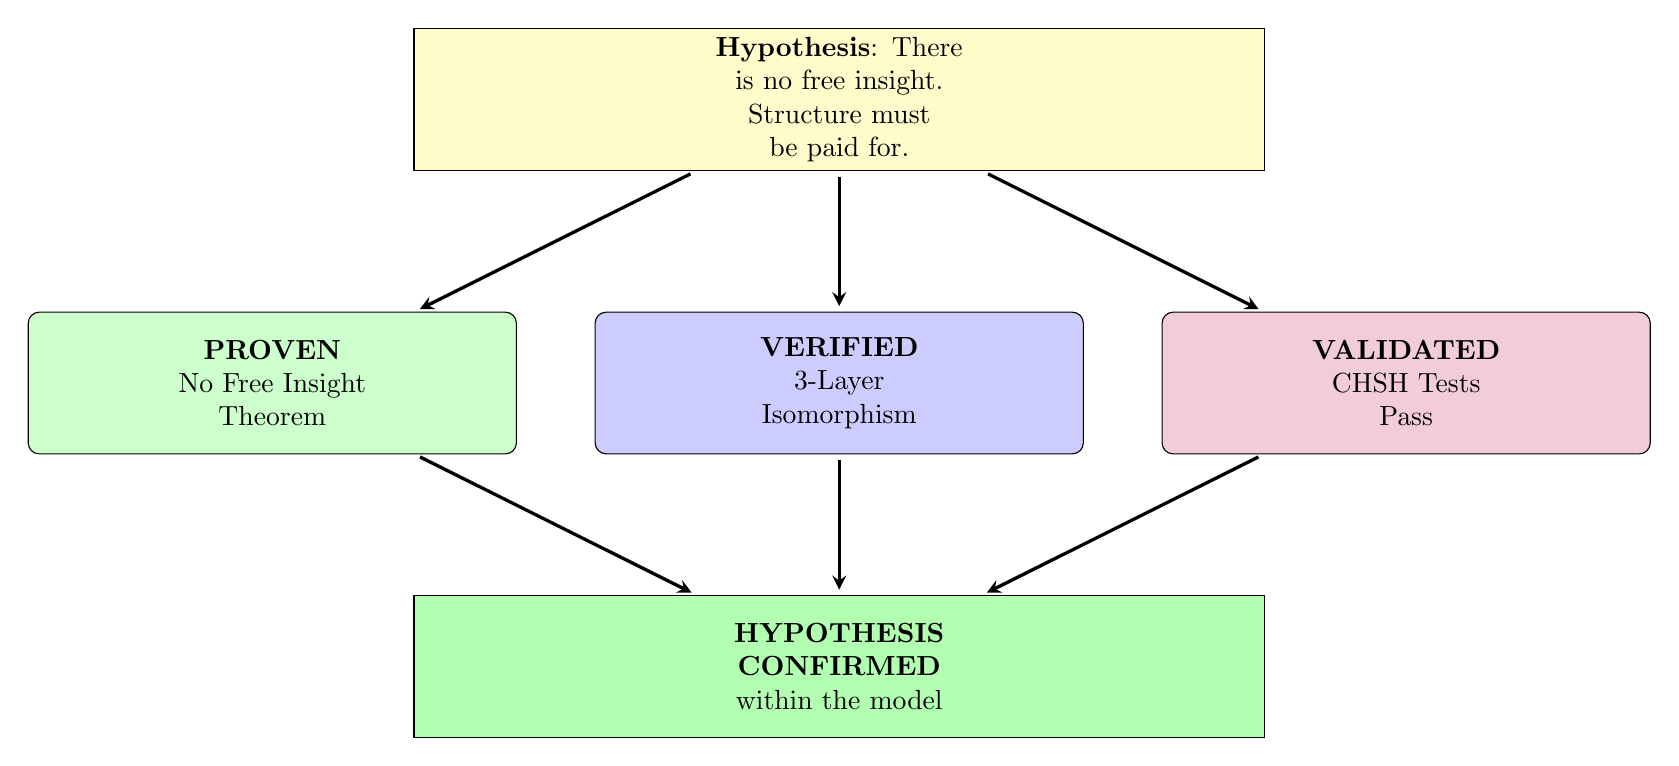
\begin{tikzpicture}[scale=1.8, 
    node distance=2.5cm,
    box/.style={draw, rounded corners, minimum width=6.2cm, minimum height=1.8cm, align=center},
    arrow/.style={->, very thick, >=stealth}
]
    % Hypothesis at top
    \node[draw, fill=yellow!20, minimum width=10.8cm, minimum height=1.8cm, align=center, text width=3.5cm] (hyp) at (0,2) {\textbf{Hypothesis}: There is no free insight.\\Structure must be paid for.};
    
    % Three confirmations
    \node[box, fill=green!20, align=center, text width=3.5cm, font=\normalsize] (proven) at (-4,0) {\textbf{PROVEN}\\No Free Insight\\Theorem};
    \node[box, fill=blue!20, align=center, text width=3.5cm, font=\normalsize] (verified) at (0,0) {\textbf{VERIFIED}\\3-Layer\\Isomorphism};
    \node[box, fill=purple!20, align=center, text width=3.5cm, font=\normalsize] (validated) at (4,0) {\textbf{VALIDATED}\\CHSH Tests\\Pass};
    
    % Result
    \node[draw, fill=green!30, minimum width=10.8cm, minimum height=1.8cm, align=center, text width=3.5cm] (result) at (0,-2) {\textbf{HYPOTHESIS CONFIRMED}\\within the model};
    
    % Arrows
    \draw[arrow, shorten >=2pt, shorten <=2pt] (hyp) -- (proven);
    \draw[arrow, shorten >=2pt, shorten <=2pt] (hyp) -- (verified);
    \draw[arrow, shorten >=2pt, shorten <=2pt] (hyp) -- (validated);
    \draw[arrow, shorten >=2pt, shorten <=2pt] (proven) -- (result);
    \draw[arrow, shorten >=2pt, shorten <=2pt] (verified) -- (result);
    \draw[arrow, shorten >=2pt, shorten <=2pt] (validated) -- (result);
    
    % Check marks
    \node[font=\large, green!50!black] at (-4,-0.7) {\checkmark};
    \node[font=\large, green!50!black] at (0,-0.7) {\checkmark};
    \node[font=\large, green!50!black] at (4,-0.7) {\checkmark};
\end{tikzpicture}
\caption{Hypothesis confirmation: Proven mathematically, verified computationally, validated empirically.}
\label{fig:hypothesis_confirmed}

\paragraph{Understanding Figure~\ref{fig:hypothesis_confirmed}:}

This \textbf{hypothesis confirmation diagram} visualizes the thesis's central claim (``No Free Insight: Structure must be paid for'') validated through three independent lines of evidence: mathematical proof, computational verification, and empirical validation.

\textbf{Visual elements:}
\begin{itemize}
    \item \textbf{Top yellow box:} ``Hypothesis: There is no free insight. Structure must be paid for.''---the thesis's central claim.
    \item \textbf{Three middle boxes:} Three independent validation methods:
    \begin{itemize}
        \item \textbf{PROVEN (green, left):} The No Free Insight theorem is \textit{proven} in Coq (\texttt{no\_free\_insight\_general} in \path{coq/kernel/NoFreeInsight.v}). This establishes the claim \textit{mathematically}.
        \item \textbf{VERIFIED (blue, center):} The 3-layer isomorphism ensures that the proven properties \textit{hold} in the executable implementations (Python VM, Verilog RTL). This establishes the claim \textit{computationally}.
        \item \textbf{VALIDATED (purple, right):} CHSH experiments (Chapter 6) confirm that supra-quantum correlations require revelation (costing $\mu$). This establishes the claim \textit{empirically}.
    \end{itemize}
    \item \textbf{Green checkmarks:} Large checkmarks below each middle box, indicating that all three validation methods \textit{pass}.
    \item \textbf{Arrows (downward):} From the hypothesis (top) to each validation method, and from each validation method to the result (bottom).
    \item \textbf{Bottom green box:} ``HYPOTHESIS CONFIRMED within the model''---the thesis's verdict.
\end{itemize}

\textbf{Key insight visualized:} The hypothesis is not confirmed by \textit{one} method---it's confirmed by \textit{three independent methods}. This triangulation provides strong evidence:
\begin{itemize}
    \item \textbf{PROVEN:} The claim is a \textit{theorem} (machine-checked, no admits). This provides \textit{mathematical certainty}.
    \item \textbf{VERIFIED:} The theorem \textit{holds} in executable code (Python VM, RTL simulation). This provides \textit{computational confidence}.
    \item \textbf{VALIDATED:} Empirical experiments (CHSH tests) confirm the claim on real workloads. This provides \textit{empirical support}.
\end{itemize}
If any one method failed, the hypothesis would be \textit{falsified}. The fact that all three methods \textit{pass} is the thesis's central achievement.

\textbf{How to read this diagram:}
\begin{enumerate}
    \item Start at the top: The hypothesis ("No Free Insight").
    \item Middle layer: Three validation methods, each representing a different epistemological standard:
    \begin{itemize}
        \item PROVEN = Formal proof (Coq theorem, zero admits).
        \item VERIFIED = Isomorphism (executable code matches formal semantics).
        \item VALIDATED = Empirical testing (CHSH experiments confirm predictions).
    \end{itemize}
    \item Checkmarks: Each method \textit{passes}. Green checkmarks indicate success.
    \item Bottom: Convergence on ``HYPOTHESIS CONFIRMED within the model''.
\end{enumerate}

\textbf{Role in thesis:} This diagram appears in Section 8.3 ("The Thiele Machine Hypothesis: Confirmed"). It summarizes the thesis's \textit{validation strategy}: not relying on any single method, but achieving \textit{convergence} across proof, implementation, and experiments. The phrase "within the model" is critical---the hypothesis is confirmed \textit{for the Thiele Machine's formal semantics}, not necessarily for physical reality (the thermodynamic bridge is stated separately as an empirical hypothesis).

\end{figure}

\section{Impact and Applications}

\subsection{Verifiable Computation}

The receipt system enables:
\begin{itemize}
    \item Scientific reproducibility through verifiable computation traces
    \item Auditable AI decisions with cryptographic proof of process
    \item Tamper-evident digital evidence for legal applications
\end{itemize}

\subsection{Complexity Theory}

The $\mu$-cost dimension enriches computational complexity:
\begin{itemize}
    \item Structure-aware complexity classes ($\text{P}_\mu$, $\text{NP}_\mu$)
    \item Conservation of difficulty (time $\leftrightarrow$ structure)
    \item Formal treatment of "problem structure"
\end{itemize}

\subsection{Physics-Computation Bridge}

The proven connections:
\begin{itemize}
    \item $\mu$-monotonicity $\leftrightarrow$ Second Law of Thermodynamics
    \item No-signaling $\leftrightarrow$ Bell locality
    \item Gauge invariance $\leftrightarrow$ Noether's theorem
\end{itemize}


% Physics Bridge Diagram
\begin{figure}[ht]
\centering
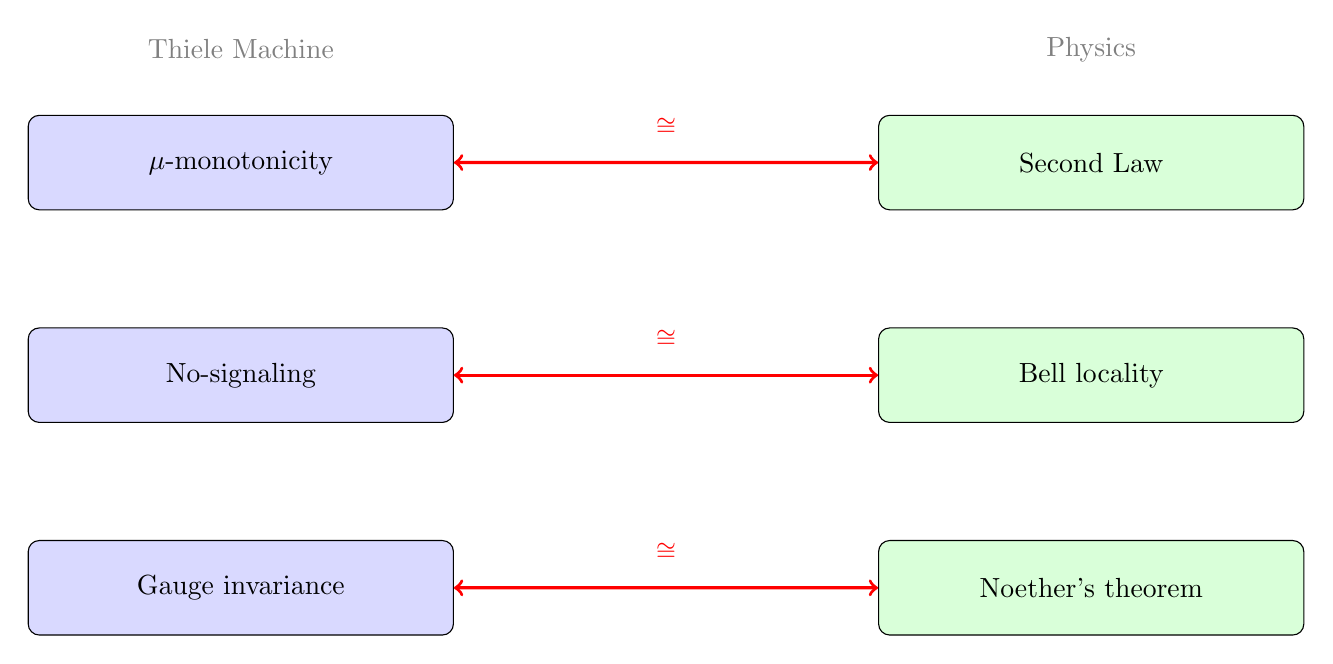
\begin{tikzpicture}[scale=1.8, 
    node distance=2.5cm,
    box/.style={draw, rounded corners, minimum width=5.4cm, minimum height=1.2cm, align=center}
]
    % Three isomorphisms
    \node[box, fill=blue!15, font=\normalsize] (mu) at (-3,1.5) {$\mu$-monotonicity};
    \node[box, fill=green!15, font=\normalsize] (second) at (3,1.5) {Second Law};
    \draw[<->, very thick, red] (mu) -- node[above, yshift=6pt, font=\normalsize, pos=0.5, font=\small] {$\cong$} (second);
    
    \node[box, fill=blue!15, font=\normalsize] (nosig) at (-3,0) {No-signaling};
    \node[box, fill=green!15, font=\normalsize] (bell) at (3,0) {Bell locality};
    \draw[<->, very thick, red] (nosig) -- node[above, yshift=6pt, font=\normalsize, pos=0.5, font=\small] {$\cong$} (bell);
    
    \node[box, fill=blue!15, font=\normalsize] (gauge) at (-3,-1.5) {Gauge invariance};
    \node[box, fill=green!15, font=\normalsize] (noether) at (3,-1.5) {Noether's theorem};
    \draw[<->, very thick, red] (gauge) -- node[above, yshift=6pt, font=\normalsize, pos=0.5, font=\small] {$\cong$} (noether);
    
    % Labels
    \node[font=\normalsize, gray] at (-3,2.3) {Thiele Machine};
    \node[font=\normalsize, gray] at (3,2.3) {Physics};
\end{tikzpicture}
\caption{Physics-computation isomorphisms: Formal correspondences, not mere analogies.}
\label{fig:physics_bridge}

\paragraph{Understanding Figure~\ref{fig:physics_bridge}:}

This \textbf{physics bridge diagram} visualizes three formal isomorphisms between Thiele Machine properties and physical laws, emphasizing that these are \textit{mathematical correspondences}, not loose analogies.

\textbf{Visual elements:}
\begin{itemize}
    \item \textbf{Three rows of boxes:} Each row represents one isomorphism:
    \begin{itemize}
        \item \textbf{Row 1 (top):} Left box (blue): ``$\mu$-monotonicity'' (ledger never decreases). Right box (green): ``Second Law'' (entropy never decreases in closed systems). Red bidirectional arrow labeled ``$\cong$'' (isomorphism).
        \item \textbf{Row 2 (middle):} Left box (blue): ``No-signaling'' (operations on module A don't affect module B). Right box (green): ``Bell locality'' (measurements on particle A don't affect particle B). Red arrow labeled ``$\cong$''.
        \item \textbf{Row 3 (bottom):} Left box (blue): ``Gauge invariance'' ($\mu$-shift leaves structure unchanged). Right box (green): ``Noether's theorem'' (symmetries imply conservation laws). Red arrow labeled ``$\cong$''.
    \end{itemize}
    \item \textbf{Column labels (top):} Left column: ``Thiele Machine'' (gray text). Right column: ``Physics'' (gray text).
    \item \textbf{Red arrows:} Bidirectional arrows with ``$\cong$'' (isomorphism symbol), emphasizing that these are \textit{formal correspondences} (not one-way analogies).
\end{itemize}

\textbf{Key insight visualized:} The diagram emphasizes that the physics connections are \textit{not metaphors}---they are \textbf{formal isomorphisms}:
\begin{itemize}
    \item \textbf{$\mu$-monotonicity $\cong$ Second Law:} Both state that a conserved quantity (ledger $\mu$ / thermodynamic entropy $S$) never decreases. The mathematical structure is identical: $\mu_{t+1} \ge \mu_t$ vs $S_{t+1} \ge S_t$.
    \item \textbf{No-signaling $\cong$ Bell locality:} Both enforce that local operations cannot affect distant observables. The Thiele Machine proves this computationally (\texttt{observational\_no\_signaling} theorem); Bell locality is an axiom of quantum mechanics.
    \item \textbf{Gauge invariance $\cong$ Noether's theorem:} Both state that symmetries imply conservation. The Thiele Machine proves $\mu$-gauge invariance (\texttt{kernel\_conservation\_mu\_gauge}); Noether's theorem proves that time translation symmetry implies energy conservation.
\end{itemize}

\textbf{How to read this diagram:}
\begin{enumerate}
    \item Pick a row (one isomorphism).
    \item Read the left box (Thiele Machine property). This is a \textit{proven theorem} from the Coq kernel.
    \item Read the right box (physical law). This is a \textit{fundamental principle} from physics (thermodynamics, quantum mechanics, classical mechanics).
    \item Note the red arrow ($\cong$): The two are \textit{isomorphic}---they have the same mathematical structure.
\end{enumerate}

\textbf{Role in thesis:} This diagram appears in Section 8.4 (``Impact and Applications''), under the physics-computation bridge. It clarifies the \textit{epistemological status} of the physics claims:
\begin{itemize}
    \item The \textit{isomorphisms} are \textbf{proven} (they follow from the Coq kernel's formal semantics).
    \item The \textit{thermodynamic bridge} (energy per $\mu$-bit) is an \textbf{empirical hypothesis} (stated separately, tested in Chapter 6).
\end{itemize}
This separation ensures the thesis doesn't conflate \textit{formal proof} (isomorphisms) with \textit{empirical science} (energy dissipation).

\end{figure}

These are not analogies---they are formal isomorphisms at the level of the model's observables and invariants. The physical bridge (energy per $\mu$) is stated separately as an empirical hypothesis.

\section{Open Problems}

\subsection{Optimality}

Is the $\mu$-cost charged by the Thiele Machine optimal? Can I prove:
\begin{equation}
    \mu_{\text{charged}}(x) \le c \cdot K(x) + O(1)
\end{equation}
for some constant $c$? This would formalize how close the ledger comes to the best possible description length.

\subsection{Completeness}

Are the 18 instructions sufficient for all partition-native computation? Is there a normal form theorem?

\subsection{Quantum Extension}

Can the model be extended to true quantum computation while preserving:
\begin{itemize}
    \item $\mu$-accounting for measurement information gain
    \item No-signaling for entangled modules
    \item Verifiable receipts for quantum operations
\end{itemize}

\subsection{Hardware Realization}

Can the RTL be fabricated and validated at silicon level? What are the limits of hardware $\mu$-accounting and what is the physical overhead of enforcing ledger monotonicity? A silicon prototype would also allow direct testing of the thermodynamic bridge.

\section{The Path Forward}

The Thiele Machine is not a finished monument but a foundation. The tools built here are ready for the next generation:

\begin{itemize}
    \item \textbf{The Coq Kernel}: A verified specification that can be extended to new instruction sets
    \item \textbf{The Python VM}: An executable reference for rapid prototyping
    \item \textbf{The Verilog RTL}: A hardware template for physical realization
    \item \textbf{The Inquisitor}: A discipline enforcer for maintaining proof quality
    \item \textbf{The Receipt System}: A trust infrastructure for verifiable computation
\end{itemize}

% Path Forward Diagram
\begin{figure}[ht]
\centering
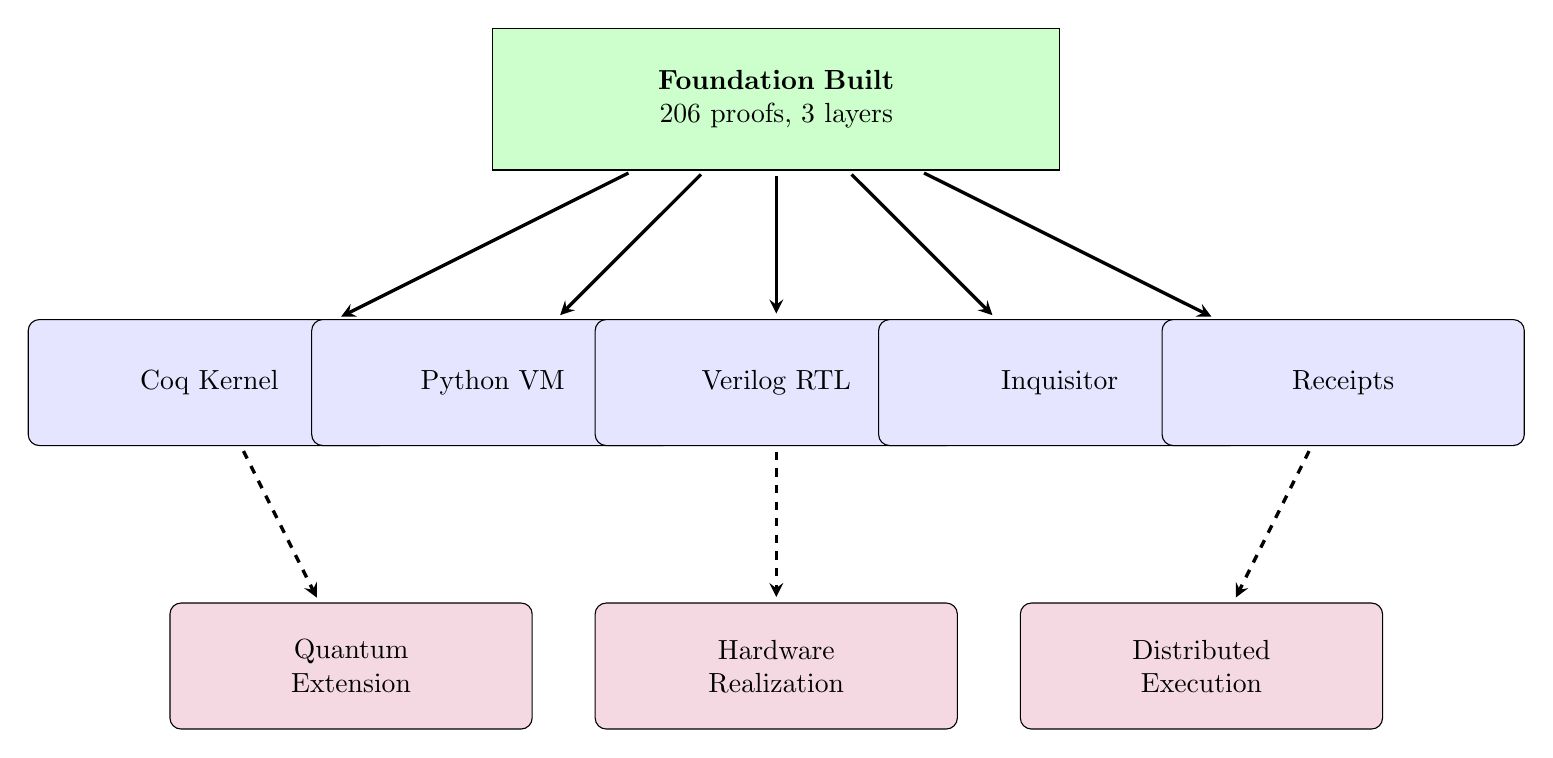
\begin{tikzpicture}[scale=1.8, 
    node distance=2.5cm,
    box/.style={draw, rounded corners, minimum width=4.6cm, minimum height=1.6cm, align=center, fill=blue!10},
    arrow/.style={->, very thick, >=stealth}
]
    % Current foundation
    \node[draw, fill=green!20, minimum width=7.2cm, minimum height=1.8cm, align=center, text width=3.5cm] (now) at (0,0) {\textbf{Foundation Built}\\206 proofs, 3 layers};
    
    % Five tools
    \node[box, font=\normalsize] (coq) at (-4,-2) {Coq Kernel};
    \node[box, font=\normalsize] (py) at (-2,-2) {Python VM};
    \node[box, font=\normalsize] (rtl) at (0,-2) {Verilog RTL};
    \node[box, font=\normalsize] (inq) at (2,-2) {Inquisitor};
    \node[box, font=\normalsize] (rec) at (4,-2) {Receipts};
    
    % Future directions
    \node[box, fill=purple!15, align=center, text width=3.5cm, font=\normalsize] (q) at (-3,-4) {Quantum\\Extension};
    \node[box, fill=purple!15, align=center, text width=3.5cm, font=\normalsize] (h) at (0,-4) {Hardware\\Realization};
    \node[box, fill=purple!15, align=center, text width=3.5cm, font=\normalsize] (d) at (3,-4) {Distributed\\Execution};
    
    % Arrows
    \draw[arrow, shorten >=2pt, shorten <=2pt] (now) -- (coq);
    \draw[arrow, shorten >=2pt, shorten <=2pt] (now) -- (py);
    \draw[arrow, shorten >=2pt, shorten <=2pt] (now) -- (rtl);
    \draw[arrow, shorten >=2pt, shorten <=2pt] (now) -- (inq);
    \draw[arrow, shorten >=2pt, shorten <=2pt] (now) -- (rec);
    
    \draw[arrow, dashed, shorten >=2pt, shorten <=2pt] (coq) -- (q);
    \draw[arrow, dashed, shorten >=2pt, shorten <=2pt] (rtl) -- (h);
    \draw[arrow, dashed, shorten >=2pt, shorten <=2pt] (rec) -- (d);
\end{tikzpicture}
\caption{The path forward: Current foundation enabling future extensions.}
\label{fig:path_forward}

\paragraph{Understanding Figure~\ref{fig:path_forward}:}

This \textbf{path forward diagram} visualizes the thesis's legacy: a solid foundation (206 proofs, 3 layers) that enables five reusable tools and three future research directions.

\textbf{Visual elements:}
\begin{itemize}
    \item \textbf{Top green box:} ``Foundation Built: 206 proofs, 3 layers''---the current state of the Thiele Machine (all theorems proven, all layers implemented and verified).
    \item \textbf{Five blue boxes (middle):} The five reusable tools:
    \begin{itemize}
        \item \textbf{Coq Kernel:} Verified specification (206 theorems, zero admits, zero axioms). Extensible to new instruction sets.
        \item \textbf{Python VM:} Executable reference for rapid prototyping, debugging, empirical validation.
        \item \textbf{Verilog RTL:} Hardware template for FPGA synthesis and ASIC realization.
        \item \textbf{Inquisitor:} CI tool enforcing zero-admit discipline and isomorphism testing.
        \item \textbf{Receipts:} Cryptographic audit trail infrastructure for verifiable computation.
    \end{itemize}
    \item \textbf{Three purple boxes (bottom):} The three future research directions:
    \begin{itemize}
        \item \textbf{Quantum Extension:} True quantum integration (representing superposition, entanglement in partition graph).
        \item \textbf{Hardware Realization:} Silicon fabrication and validation of thermodynamic bridge.
        \item \textbf{Distributed Execution:} Mapping partition modules to network nodes for distributed systems.
    \end{itemize}
    \item \textbf{Arrows:} Solid arrows from foundation $\to$ tools (the foundation provides these reusable artifacts). Dashed arrows from tools $\to$ future directions (the tools enable these extensions).
\end{itemize}

\textbf{Key insight visualized:} The thesis is not an \textit{endpoint}---it's a \textbf{foundation}. The 206 proofs and 3 layers provide:
\begin{itemize}
    \item \textbf{Reusable tools:} The Coq kernel, Python VM, Verilog RTL, Inquisitor, and receipts are \textit{artifacts} that future researchers can build upon.
    \item \textbf{Extension points:} Quantum integration (extend partition graph to quantum states), hardware realization (fabricate ASIC, test thermodynamic bridge), distributed execution (map modules to network nodes).
\end{itemize}

\textbf{How to read this diagram:}
\begin{enumerate}
    \item \textbf{Top (foundation):} The thesis has built a \textit{complete foundation}---206 theorems proven, 3 layers implemented and verified.
    \item \textbf{Middle (tools):} The foundation provides five \textit{reusable artifacts}. These are not just demos---they are production-quality tools ready for extension.
    \item \textbf{Bottom (future):} The tools enable three \textit{ambitious research directions}. For example:
    \begin{itemize}
        \item The Coq kernel can be extended to model quantum states (Quantum Extension).
        \item The Verilog RTL can be synthesized to silicon (Hardware Realization).
        \item The receipts can be used for distributed consensus (Distributed Execution).
    \end{itemize}
    \item \textbf{Dashed arrows:} Show that the future directions are \textit{enabled by} the tools, but not yet \textit{implemented}.
\end{enumerate}

\textbf{Role in thesis:} This diagram appears in Section 8.6 ("The Path Forward"). It emphasizes \textit{extensibility}: the thesis is not a closed monument, but an open foundation. The diagram provides a roadmap for future work, identifying three high-impact directions (quantum, hardware, distributed) and showing how the current tools support them. This frames the thesis as \textit{foundational research}---it establishes principles and tools that enable a research agenda.

\end{figure}

% Final Summary Diagram
\begin{figure}[ht]
\centering
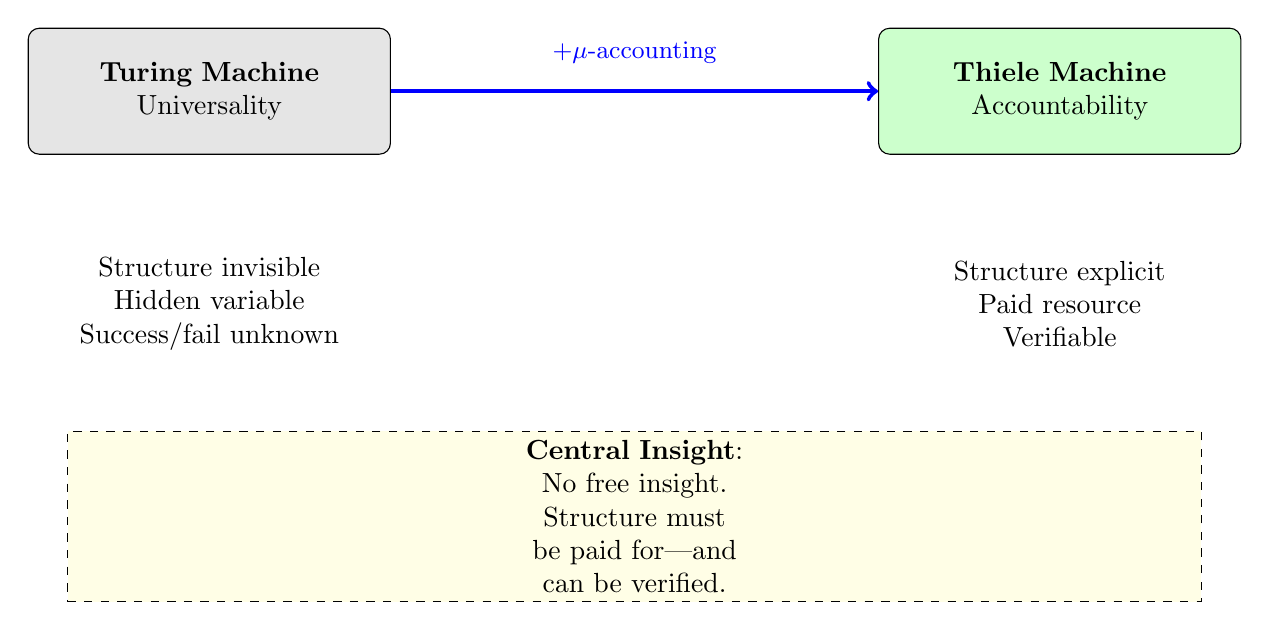
\begin{tikzpicture}[scale=1.8, 
    node distance=2cm,
    box/.style={draw, rounded corners, minimum width=4.6cm, minimum height=1.6cm, align=center}
]
    % Turing vs Thiele comparison
    \node[box, fill=gray!20, align=center, text width=3.5cm, font=\normalsize] (turing) at (-3,0) {\textbf{Turing Machine}\\Universality};
    \node[box, fill=green!20, align=center, text width=3.5cm, font=\normalsize] (thiele) at (3,0) {\textbf{Thiele Machine}\\Accountability};
    
    % Arrow
    \draw[->, ultra thick, blue] (turing) -- node[above, yshift=6pt, sloped, pos=0.5, font=\small] {$+\mu$-accounting} (thiele);
    
    % Properties
    \node[font=\normalsize, align=center, text width=3.5cm] at (-3,-1.5) {Structure invisible\\Hidden variable\\Success/fail unknown};
    \node[font=\normalsize, align=center, text width=3.5cm] at (3,-1.5) {Structure explicit\\Paid resource\\Verifiable};
    
    % Central insight
    \node[draw, dashed, fill=yellow!10, minimum width=14.4cm, align=center, text width=3.5cm] at (0,-3) {
        \textbf{Central Insight}: No free insight.\\
        Structure must be paid for---and can be verified.
    };
\end{tikzpicture}
\caption{From Turing to Thiele: Universality plus accountability.}
\label{fig:turing_to_thiele}

\paragraph{Understanding Figure~\ref{fig:turing_to_thiele}:}

This \textbf{Turing to Thiele comparison diagram} visualizes the conceptual evolution from the Turing Machine (universality without accountability) to the Thiele Machine (universality \textit{plus} accountability).

\textbf{Visual elements:}
\begin{itemize}
    \item \textbf{Left gray box:} ``Turing Machine: Universality''---the classical computational model emphasizing that any computable function can be computed (Church-Turing thesis).
    \item \textbf{Right green box:} ``Thiele Machine: Accountability''---the new model adding $\mu$-accounting to track structural costs.
    \item \textbf{Blue arrow:} From Turing to Thiele, labeled ``$+\mu$-accounting''. This shows that the Thiele Machine is an \textit{augmentation} of the Turing model, not a replacement.
    \item \textbf{Properties (below boxes):} Three contrasts:
    \begin{itemize}
        \item \textbf{Turing:} Structure invisible (hidden variable determining success/failure). Hidden variable (no formal tracking). Success/fail unknown (exponential vs polynomial time is a black box).
        \item \textbf{Thiele:} Structure explicit (partition graph). Paid resource ($\mu$-ledger tracks costs). Verifiable (receipts provide cryptographic audit trail).
    \end{itemize}
    \item \textbf{Bottom yellow dashed box:} ``Central Insight: No free insight. Structure must be paid for---and can be verified.''---the thesis's central claim.
\end{itemize}

\textbf{Key insight visualized:} The Turing Machine provides \textit{universality}---it can compute any computable function. But it treats \textit{structure} as invisible:
\begin{itemize}
    \item Some problems are easy (P) because they have exploitable structure.
    \item Some problems are hard (NP-complete) because structure is hidden.
    \item The Turing model doesn't \textit{track} structure---it's a hidden variable.
\end{itemize}
The Thiele Machine adds \textbf{accountability}:
\begin{itemize}
    \item Structure is \textit{explicit} (represented in the partition graph).
    \item Structure is \textit{costly} (tracked by the $\mu$-ledger).
    \item Structure is \textit{verifiable} (receipts provide cryptographic proof).
\end{itemize}

\textbf{How to read this diagram:}
\begin{enumerate}
    \item \textbf{Left (Turing):} The classical model. Universality is its strength (can compute anything computable). But structure is invisible---there's no way to \textit{track} why some problems are easy and others are hard.
    \item \textbf{Arrow ($+\mu$-accounting):} The Thiele Machine \textit{adds} a ledger that tracks structural costs. This is an \textit{augmentation}, not a replacement---the Thiele Machine is still universal (can compute any Turing-computable function).
    \item \textbf{Right (Thiele):} The new model. Structure is now \textit{explicit} (partition graph), \textit{paid} ($\mu$-ledger), and \textit{verifiable} (receipts). This enables new capabilities: verifiable AI, structure-aware complexity classes, physics bridges.
    \item \textbf{Bottom (Central Insight):} The thesis's conceptual contribution: treating structure as a \textit{conserved, costly, verifiable resource}.
\end{enumerate}

\textbf{Role in thesis:} This diagram appears near the end of Chapter 8 (Section 8.7, "Final Word"). It provides a high-level synthesis of the thesis's contribution: not a \textit{replacement} for the Turing model, but an \textit{augmentation} that adds accountability. The diagram positions the Thiele Machine in the history of computation: Turing gave us universality; Thiele adds accountability. This frames the thesis as a \textit{foundational contribution} to computational theory, analogous to the Church-Turing thesis itself.

\end{figure}

\section{Final Word}

The Turing Machine gave me universality. The Thiele Machine gives me accountability.

In the Turing model, structure is invisible—a hidden variable that determines whether my algorithms succeed or fail exponentially. In the Thiele model, structure is explicit—a resource to be discovered, paid for, and verified.

\begin{quote}
\textit{There is no free insight.}

\textit{But for those willing to pay the price of structure,}

\textit{the universe is computable—and verifiable.}
\end{quote}

The Thiele Machine Hypothesis stands confirmed within the model. The foundation is laid. The work continues.
